\chapter{Nested Class Modularity in Squeak}
In this chapter, we describe the main concept of our work: classes as class members. Similar concepts are part of programming languages like Java, Ruby, Python, and Newspeak. Our concept follows closely the Newspeak notion of nested classes, but without making invasive changes to the Smalltalk programming language.

\section{Nested Classes}
In Smalltalk, every object is an instance of a class, defining the object's instance variables and the messages it understands. Consequently, a class is also an instance of its so-called meta class. Every meta class is an instance of \texttt{Metaclass} (Figure~\ref{fig:impl_squeak_meta}). In the remainder of this work, we denote the meta class of a class \texttt{C} by \texttt{C class}. Every Smalltalk image has a \texttt{globals} dictionary, mapping symbols to class objects, so that references to classes can be resolved at compile time. This implies that all references to classes are early bound.

\begin{wrapfigure}{l}{0.5\textwidth}
	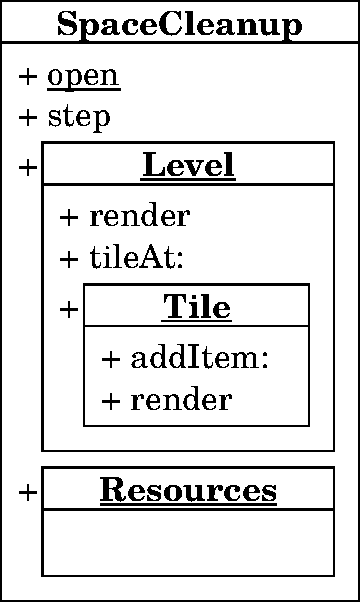
\includegraphics[scale=0.75]{nested_notation.pdf}
	\centering
	\caption{Nested Classes Example}
	\label{fig:concept_nested_notation}
\end{wrapfigure}

Our system extends the Smalltalk class organization as follows: in addition to regular methods, we introduce the concept of \emph{class generator methods}. Such a method generates a class and is associated with a set $I$ of instance methods and a set $C$ of class methods. Whenever the method is invoked, the system first executes the method body, then adds $I$ to resulting class and $C$ to resulting meta class, and finally returns the resulting class. For performance reasons, our system also caches the result, meaning that a class is not generated twice.

\paragraph{Details}
Class generator methods are only allowed as class-side methods. Instance-side class generator methods seem to provide neglectable benefits and make the implementation of our system more complicated. We provide an in-depth explanation of instance-side class generator methods in the Section~\ref{sec:future_inst_side}.

A class generated by a class generator method is anonymous: it is not listed in the \texttt{globals} dictionary and can only be referenced using message sends to its enclosing class\footnote{It can also be references by sending the \texttt{class} method to one of its instances}. Consequently, its name is a concatenation of all class names on the path from the top-level class to class in question.


\paragraph{Notation and Example}
Figure~\ref{fig:concept_nested_notation} shows an example of nested classes in Squeak. \texttt{A} is a top-level class, i.e., it is part of the \texttt{globals} dictionary and known everywhere in the system; it can be referenced by just writing the identifier \texttt{A}. \texttt{A} has one instance method \texttt{m2} and two class methods \texttt{m1} and \texttt{B}. In accordance with UML notation, class-side method selectors are underlined. 

\texttt{A class>>B} is a class generator method that is associated with a set of instance methods $\{\}$ and a set of class methods $\{\mbox{\texttt{foo}, \texttt{B}}\}$. The name of the class it generates is \texttt{A B}, which is in that case also a valid Smalltalk code expression that evaluates to the generated class. \texttt{A class>>B class>>C} is a class generator method that generates \texttt{A B C}. Note, that we use the \texttt{>>} notation to not only reference methods but also the classes they generate, in case they are class generator methods.

%\begin{figure}[!htp]
%	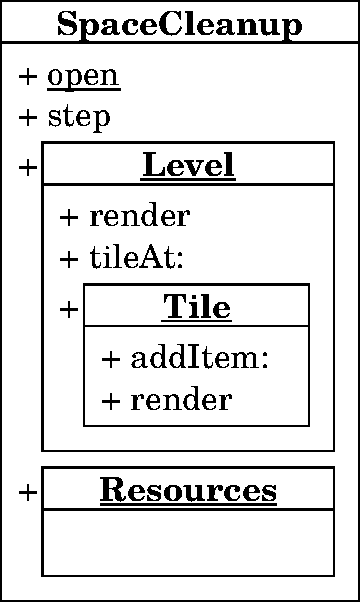
\includegraphics[scale=0.5]{nested_notation.pdf}
%	\centering
%	\caption{Nested Classes Example}
%	\label{fig:concept_nested_notation}
%\end{figure}

\section{Accessing the Lexical Scope}
It is sometimes necessary to access a method's lexical scope (i.e., the enclosing classes), in order to send messages to enclosing classes. For this reason, our system introduces new keywords, in addition to \texttt{self} and \texttt{super}, which are already present in every Smalltalk dialect. Figure~\ref{fig:concept_keywords} gives an overview of all method lookup-related keywords in the system.

\begin{figure}[!hbp]
	\centering
	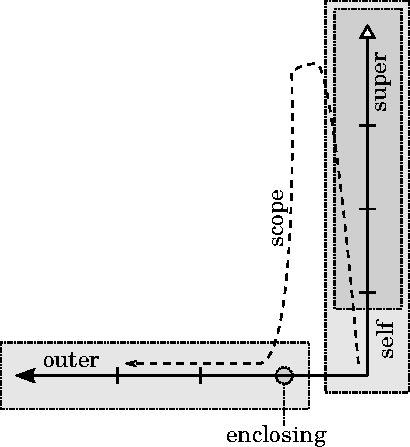
\includegraphics[scale=1]{lookup_keywords.pdf}
	\caption{Keywords for access to superclass and lexical scope.}
	\label{fig:concept_keywords}
\end{figure}

\paragraph{\texttt{self} Keyword}
This keyword is used make a message send within an object. The receiver is the same object as the sender and the lookup starts at the (polymorphic) class of the receiver. If that class does not provide a corresponding method, the lookup continues in the superclass hierarchy. If no class in the superclass has a corresponding method, a \texttt{MethodNotUnderstood} error is raised.

\paragraph{\texttt{super} Keyword}
This keyword is also used to make a message send within an object. Again, the receiver is the same object as the sender, but the lookup starts at superclass of the sender's method class. Note, that \texttt{super} is bound to the superclass of the method class, not the superclass of the receiver's class.

\paragraph{\texttt{enclosing} Keyword}
\todo{Binding of arguments for parameterized classes.}
This keyword is used to make a message send to the class that contains the current current. Consider, for example, that we want to send a message \texttt{foo} to class \texttt{A B} within \texttt{A class>>B class>>C>>m5} in Figure~\ref{fig:concept_nested_notation}. Either one of the following two statements works in this case.

\begin{itemize}
	\item \texttt{A B foo.}
	\item \texttt{enclosing foo.}
\end{itemize}

\texttt{enclosing} is a keyword that evaluates to the method owner's enclosing class upon method compilation. Note, that \texttt{enclosing} is bound to the method's lexical scope, not the receiver's lexical scope.

Figure~\ref{fig:concept_lexical_thisouter} illustrates how \texttt{enclosing} is bound. In \texttt{B1 class>>C class>>bar1}, \texttt{enclosing} is bound to \texttt{B1}. In contrast, \texttt{B2 class>>C class>>bar2} binds \texttt{enclosing} to \texttt{B2}. Consequently, \texttt{B1 C bar1} calls \texttt{B1 foo} and so does \texttt{B2 C bar1}, even though the receiver of \texttt{bar1} is an instance of \texttt{B2 C class} and not \texttt{B1 C class} in the latter case. Note, that \texttt{B2 C bar2} calls \texttt{B2 foo}, because \texttt{bar2}'s lexically enclosing class is \texttt{B2}.

\begin{figure}[!htp]
	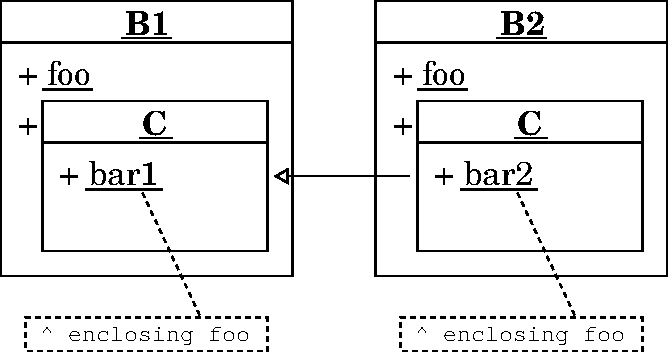
\includegraphics[scale=0.75]{nested_lexical1.pdf}
	\centering
	\caption{Binding of \texttt{enclosing} to method's lexical scope.}
	\label{fig:concept_lexical_thisouter}
\end{figure}

Note, that \texttt{enclosing} can be used for meta programming purposes; however, it should be avoided in general. Our system also provides a \texttt{scope} keyword that should be used instead.

\paragraph{\texttt{enclosing} Method}
In addition to \texttt{enclosing}, every class in the system has a method \texttt{enclosing} that returns the enclosing class of the receiver\footnote{The enclosing class of an object that is not a class is its class' enclosing class.}, making it possible to send messages to enclosing classes which are more than one level away. If, for example, in Figure~\ref{fig:concept_nested_notation}, \texttt{A class>>B class>>C>>bar} wants to send the message \texttt{m1} to \texttt{A}, either one of the following two statements works.

\begin{itemize}
	\item \texttt{A m1.}
	\item \texttt{enclosing enclosing m1.}
\end{itemize}

Again, the method \texttt{enclosing} should be avoided in general, but is useful to implement parts of our system with code written in the system itself.

\paragraph{\texttt{outer} Keyword}
The method \texttt{enclosing} can be used to traverse the the lexical scope of a class. Arbitrarily many \texttt{enclosing} sends can be chained, as long as the respective receiver still has an enclosing class and is, therefore, not a top-level class. Arguably, this can result in verbose and complicated code, and is at the very least questionable with regards to the law of demeter.

In addition to \texttt{enclosing}, the system provides the \texttt{outer} keyword, bound to the method's lexical scope. Whenever a message is sent to \texttt{outer}, the message is first interpreted as a send to \texttt{enclosing}. If that message send fails, the message is sent to \texttt{enclosing enclosing}, and, eventually, to the top-level class, if no other class in the lexical scope understands the message. If even that message send is not understood, the selector is looked up in the \texttt{globals} dictionary. If the selector is absent, a \texttt{MessageNotUnderstood} error is raised.

\texttt{outer} is similar to \texttt{super}, with the difference that \texttt{outer} does a horizontal lookup (lexical scope) and \texttt{super} does a vertical lookup (superclass chain). Note, that messages sent to \texttt{outer} are sent to an object different from \texttt{self}.

\paragraph{\texttt{scope} Keyword}
This keyword combines \texttt{super} and \texttt{outer}: a message sent to \texttt{scope} is first treated as a \texttt{self} send. If the message is not understood, it is treated as an \texttt{outer} send.

Our system essentially first looks up the methods in \texttt{self}, then in the superclass hierarchy, and then in the lexical scope. This is also how the method lookup in Java works, also known as \emph{comb semantics}\todo{Add reference:  Smith, W.R.: NewtonScript: Prototypes on the Palm, pp. 109 – 139. SpringerVerlag (1999), in Prototype-Based Programming: Concepts, Languages and Applications, Noble, Taivalsaari and Moore, editors}. Newspeak uses a different lookup: it first looks for a method in the receiver's class, then in the lexical scope, and finally in superclass hierarchy~\cite{bracha:modules_as_objects}.

The statement \texttt{enclosing enclosing m1} in the previous example can also be written as \texttt{scope m1}. If the method \texttt{m1} would now be moved to its enclosing class (if it had one), the lookup would still succeed. However, \texttt{scope} exposes the risk of accidentially capturing method names in superclasses or the lexical chain.

\paragraph{Implicit \texttt{scope} Receiver}
In our system, references to globals are in fact message sends with \texttt{scope} as implicit receiver. This makes it easier for Smalltalk programmers to write code in our system, even if they do not know about \texttt{enclosing} and \texttt{scope}. It also makes the code less verbose and easier to read.

Whenever code references an identifier that is not a temporary variable, not an instance variable, and not a \emph{special} object \footnote{\texttt{self}, \texttt{super}, \texttt{thisContext}, \texttt{scope}, \texttt{outer}, \texttt{enclosing}}, the compiler replaces that identifier with a message send to \texttt{scope}.

Consider, for example, that we want to reference class \texttt{A B} within \texttt{A class>>B class>>C>>bar} in Figure~\ref{fig:concept_nested_notation}. Either one of the following two statements works in this case.

\begin{itemize}
	\item \texttt{A B.}
	\item \texttt{enclosing.}
	\item \texttt{enclosing enclosing B.}
	\item \texttt{outer B.}
	\item \texttt{scope B.}
	\item \texttt{B.}
\end{itemize}

In this example, we used the implicit \texttt{scope} receiver for class lookup, which is in our opinion the most useful case. However, any method in \texttt{self}, the lexical scope, or the superclass hierarchy can in fact be looked up this way. One can argue that this is bad practice and should be forbidden for methods that are not class generator methods. However, it is allowed in Newspeak and other programming languages like Java, and seems to work well, as long as the programmer is aware of how the method lookup works. Note, that only unary messages can have an implicit \texttt{scope} receiver, since we would have to change the Smalltalk syntax otherwise.

\section{Parameterized Classes}
All examples shown in the previous section use unparameterized classes, i.e., class generator methods are always unary. Class generator method can, however, also have binary selectors or selectors with a higher arity. For memory conservation reasons, these classes are then no longer cached.

Parameterized classes can be used to make modules externally configurable or to implement mixins. We will present some conrete use cases in Section~\ref{sec:usecases}.

The arguments passed to a parameterized class generator method are considered when a message is sent to \texttt{enclosing}. At first, the system tries to send the message to the enclosing class. If that fails, the system checks if the selector corresponds to one of the parameter names in the enclosing class' class generator method.
